In this section, we use the estimated parameters from the previous section to
analyze Model (\ref{model1}) and the effect of the vaccine. Some plausible
scenarios are presented, depending on the effectiveness of the vaccine,  as
well as the rate of vaccination.

In the first instance, it has been shown that the interest region of the state
variables of the system is positively invariant and the proof can be found in
Appendix B.


Now, an important concept in the analysis of the spread of diseases is the
basic reproductive number, defined as the number of secondary infections
produced by a typical infected individual, throughout his infectious period,
when in contact with a totally susceptible population. For your calculation,
and following the works in\cite{Diekmann1990, Van2002}, the basic reproduction
number for system (\ref{model1}) is (see Appendix B) \change{fix reference}

\begin{equation}\label{Rv}
    R_{V}=R_S+R_A
\end{equation}
with
\begin{eqnarray*}
    R_S &=& \frac{p\beta_S\delta_E(\mu+\delta_V+(1-\epsilon)
            \lambda_V)}{(\mu+\delta_E)(\mu+\delta_V+\lambda_V)(\mu+\alpha_S+\mu_S+\lambda_T)}
    \\
    R_A &=& \frac{(1-p) \beta_A \delta_E (\mu + \delta_V + (1-\epsilon)
            \lambda_V)}{(\mu+\delta_E)(\mu + \delta_V + \lambda_V)(\mu + \alpha_A + \mu_A)}
\end{eqnarray*}
 Note that each sum of $ R_ {V} $ represents the contribution of the symptomatic and asymptomatic infected,
 respectively, to the spread of the disease.
Following the ideas of Alexander et. al. \cite{Alexander2004}, expression for $R_V$ can be rewritten as
%
\begin{equation}\label{Rv2}
R_{V}=R_0\left(1- \frac{\epsilon \lambda_V}{(\mu+\delta_V+\lambda_V)}\right)
\end{equation}
where $R_0$ is the basic reproduction number of system without vaccine.
Note that
$\left(1- \frac{\epsilon \lambda_V}{(\mu+\delta_V+\lambda_V)}\right)<1$. Therefore, this factor which saves the
parameters corresponding to the application of the vaccine will allow us to modulate the value of $ R_0 $. In the
first instance, if $ R_0 <1 $, then $ R_V <1 $. But, if $ R_0> 1 $, we wonder if the application of the vaccine can
lower $R_V$ value below 1. In this sense, it is easy to prove that, if

\begin{equation}\label{condition1}
    \lambda_V>\frac{(R_0-1)(\mu+\delta_V)}{(\epsilon-1)R_0+1},
\end{equation}

for $\epsilon>1-(1/R_0)$, it is possible to reduce the value of $ R_V $ below one, of course with the necessary conditions in terms of vaccination. That is, there is a region in the parameter space in which it is possible to reduce the value of $ R_V $ below one, considering adequate efficacy, vaccination rate and duration of the effect of the vaccine. However, if the inequality (\ref{condition1}) is not satisfied, it will not be possible to reduce the value of $ R_V $ below 1.

To illustrate the aforementioned, Figure \ref{R0-2D} shows the regions where it is possible to reduce the value of $ R_V $. In this case, we set all the system parameters, which are given in table \ref{table1} and with $ \delta_V = 1/180 $, leaving $ \epsilon $ and $ \lambda_V $ free.

\begin{figure}[!h]
    \centering
    \includegraphics[width=1.0\textwidth, keepaspectratio]%
    {R0-2D.eps}
    \caption{%
        Shaded region corresponds to $R_V>1$
        while white region denotes when
        $R_V < 1$.
        This scenario considers a vaccine with $50$ percent
        efficacy, thus an adequate vaccination rate can drive
        $R_V$ value below one.}
\label{R0-2D}
\end{figure}
\change{improve redaction}
\textcolor{red}{
    On the other hand, vaccination policies to carry out the
application of the same is of utmost importance. Among other
factors, the vaccination rate at which the vaccine must be applied
in order to achieve a certain coverage of the population within a
certain horizon time must be considered. In this sense, we will
refer to this vaccination rate as the base vaccination rate and we
will denote it as $ \lambda_{Vbase} $ and which is a solution of
the equation:}

\begin{equation}\label{eqn:lambda_base}
    x_{coverage} = 1 - \exp(-\lambda_V T).
\end{equation}
That is, $\lambda_V$ denotes the constant vaccination rate to
cover  a fraction $x_{coverage}$ in time horizon $T$. So,
\Cref{R0_contour}, show the contour curves for $ R_0 $ considering
it as a function of the efficacy of the vaccine $ (\epsilon) $ and
of the vaccination rate $ (\delta_V) $, considering immunity times
due to the vaccine of half year .

Blue line in the graph correspond to the values of $\lambda_{Vbase}$
and we can see that with this vaccination rate, no matter how
effective the vaccine is, it is not possible to reduce the value of
$R_V$ below one. Purple lines show a scenario in which it is
possible to reduce the $R_V$ value below one, considering a vaccine
efficacy of 0.8 and a vaccination rate of 0.7. Figure shows
plausible combinations of $\epsilon$ and $\lambda_V$ values in order
to reduce the value of $R_V$ below one.

Note that a vaccine efficacy of $50$ percent or more is required so that,
with an adequate vaccination rate, the $R_V$ value can be reduced below one.

\begin{figure}[!h]
    \centering
    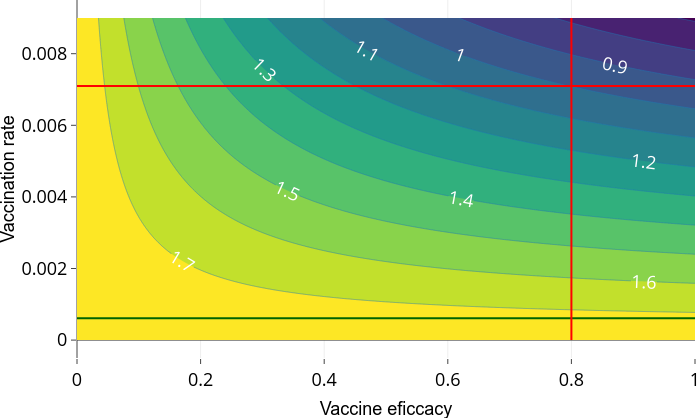
\includegraphics[scale=.50]{R0_contour.png}
    \caption{
        Contour plot  of $R_V$ like function of $\epsilon$ and
        $\lambda_V $ and with immunity average time by vaccination of half year.
        Blue line represents the value of $\lambda_{Vbase} = \num{0.000611}$,
        corresponding to a coverage $x_{coverage}=\num{0.2}$
        and a horizon time $T=\num{365}$. Purple lines show a scenario
        in which it is possible to reduce the $R_V$ value below one,
        considering a vaccine efficacy of $\epsilon =\num{0.8}$
        and a vaccination rate of $\lambda_V = num{0.7}$.
    }
    \label{R0_contour}
\end{figure}


    In the next section, the optimal control theory will be applied to propose
optimal vaccination dynamics that minimize the number of cases of symptomatic
infection and deaths due to the disease.